\documentclass[10pt]{article}
\usepackage[margin=1in]{geometry}
\usepackage{graphicx}
\usepackage{booktabs}
\usepackage{amsmath}
\usepackage{xcolor}
\usepackage{hyperref}
\hypersetup{colorlinks=true,linkcolor=blue,citecolor=blue,urlcolor=blue}
\usepackage{caption}
\usepackage{enumitem}
\usepackage{placeins}

% NOTE: de-anonymize/anonymize \author{} per venue policy before submission.
\title{\textbf{The Action Space, Not the Decomposition:\\
Why an Interpretable Mixture-of-Drives Over-Brakes---and What Makes It Drive}}
\author{Dana Kim}
\date{}

\begin{document}
\maketitle

\begin{abstract}
We study X-MoD, an interpretable Mixture-of-Drives policy for autonomous driving: a router that
arbitrates over four named drive-experts---\emph{safety, legality, comfort, efficiency}---so that the
gating weights are a human-readable account of \emph{why} the policy acts. We report three results that,
together, sharpen what ``interpretable driving'' actually delivers. \textbf{First (explanation
works):} with safety-event-aware data collection, X-MoD's safety gate becomes faithfully risk-aligned
---the gate--safety-event correlation reaches \textbf{0.80}, with the safety gate mean separating
\textbf{0.65 on safety events vs 0.04 otherwise}, at \textbf{1.5\,ms} inference. Critically, this
alignment is unlocked by \emph{data composition, not architecture}: without safety-positive samples
the identical model shows near-zero correlation. \textbf{Second (control fails under raw pedals):} when the same
interpretable policy is evaluated \emph{closed-loop} on Bench2Drive-220 it does not drive. It
collapses to a constant-brake router state, and an extensive recovery campaign---data scale-up (to
$\sim$8.5k frames / 43 routes / 9 towns), loss balancing, capacity increase, and a full structural
fork (separated mobility/brake heads, hazard-conditioned inputs, from-scratch retraining)---never
escapes a \textbf{safety/mobility seesaw}: every configuration either over-brakes (route completion
3--5\%) or under-brakes (collisions). \textbf{Third (the over-brake was the learned brake; what remains is generalization):}
the over-brake comes from the model's \emph{learned brake output}. An action head with no brake (it
\emph{cannot} over-brake) paired with a classical control stack---a PID on the predicted target speed,
a standard safety shield, and an anti-stall floor---turns the 3--5\% stall into driving. Of the five
evaluation routes only one (24211) appears in training; on the four \emph{unseen} routes the policy
\textbf{completes one at 100\% with zero collisions} (24330, robust across three traffic seeds) yet
reaches only 18--53\% on the others. The gap is \emph{scenario-dependent}, not a clean train/test
split---the lone trained route still collides, and the cleanest route is unseen---and it is not closed
by \emph{quantity} (a $11\rightarrow43$-route scaling probe leaves mean unseen completion flat), so it
is a composition/robustness gap rather than simple overfitting. We conclude that the over-brake was the learned brake output, \emph{not} the
interpretable decomposition; what remains is \emph{generalization}, which a hybrid
policy-plus-control-stack does not by itself provide.
\end{abstract}

\section{Introduction}
``Interpretable autonomous driving'' usually means that a model's internals can be \emph{read}---
attention maps, modular sub-policies, named experts. It rarely means that the readable structure has
been \emph{tested as a closed-loop controller}. These are different properties, and conflating them is
how an interpretable model earns trust it has not demonstrated.

We separate the two with a single model. X-MoD is a transparent Mixture-of-Drives: a router weights
four drive-experts (safety / legality / comfort / efficiency), and the gating vector is the model's
own explanation of its decision. We ask a deliberately blunt question: \textbf{does a transparent
value-arbitration policy that demonstrably \emph{explains} also \emph{drive}?}

Our answer is three-part and, we think, more useful than any single verdict:
\begin{itemize}[leftmargin=1.4em,itemsep=2pt]
  \item \textbf{Explanation: yes.} The safety gate measurably tracks real safety events (correlation
  0.80), and we show \emph{why}---it is unlocked by safety-event data, not by the architecture.
  \item \textbf{Control under raw pedals: no.} The same policy, evaluated closed-loop on
  Bench2Drive-220~\cite{bench2drive}, cannot reconcile safety and mobility; it sits on a seesaw
  between over-braking and colliding, and stays there across data scale, loss balancing, added
  capacity, and a structural redesign.
  \item \textbf{Control with the learned brake removed: it drives.} Zeroing the model's brake
  output (so it cannot over-brake), with braking from a standard safety shield, breaks the over-brake
  corner on the identical model and data (route completion 3--5\%~$\rightarrow$~46\%); adding a
  classical target-speed controller then drives an \emph{unseen} route to 100\% (zero collisions). The
  over-brake was the learned brake output, not the decomposition.
\end{itemize}

The contribution is to hold these results in one frame and \emph{locate} the failure precisely. The
over-brake seesaw---which survives data scale, capacity, and structural redesign while the model emits
a learned brake---is removed by zeroing that brake output (with a standard safety shield providing the
actual braking). So the over-brake was the learned brake, not the decomposition. What remains
(lateral control and scenario-dependent generalization---some unseen routes drive cleanly, others
fail) names what an interpretable arbitrator is still missing to become a controller.

\section{Related Work}
\textbf{Interpretable / privileged driving policies.} Learning by Cheating~\cite{lbc} and
Roach~\cite{roach} use privileged teachers and modular structure; we share the
transparent-arbitration motivation but evaluate \emph{whether the transparency survives as control}.
\textbf{Mixture-of-Experts policies.} X-MoD is an MoE policy with \emph{named, semantically
meaningful} experts, which is what makes its gate an explanation rather than an opaque weight.
\textbf{Explainability in driving} typically validates that an internal signal \emph{correlates} with
a concept; we do that (the safety gate), then ask the rarely-asked follow-up: does the same model
\emph{drive} closed-loop? \textbf{Closed-loop benchmarking}~\cite{bench2drive,carla,transfuser}: open-
and closed-loop scores can diverge sharply; our negative result is a concrete instance---strong
offline alignment, zero closed-loop competence.

\section{Model: X-MoD}
X-MoD is a router over four drive-experts (safety, legality, comfort, efficiency) on a shared
perceptual backbone (ResNet34 or a tinyCNN). The forward map is
$f(\text{image}_{[B,3,128,128]}, \text{ego}_{[B,2]}=[\text{speed}, \text{wp\_angle}]) \rightarrow
(\text{action}, \text{gate\_probs}, \text{experts})$, where \texttt{gate\_probs} is the router's
arbitration over the four experts and is the object of explanation. The action head performs
\textbf{direct regression of throttle / brake / steer}---a design choice we return to in
Section~\ref{sec:why} as the central confound of the negative result.

\section{Part I---Explanation Works}
\textbf{Setup.} CARLA 0.9.15~\cite{carla}, synchronized simulation; data collected with rule-based
teachers and event-driven labeling; 11{,}500 samples. We report action quality (action MSE), routing
quality (router accuracy), inference latency, and the explainability target: the correlation between
the safety gate and labeled safety events (``H3'').

\textbf{Result.} Table~\ref{tab:expl} compares three training configurations on the full sample.

\begin{table}[ht]
\centering
\caption{Explanation: routing loss and safety-event data drive gate--risk alignment.}
\label{tab:expl}
\begin{tabular}{lrrrr}
\toprule
Run & Action MSE & Router Acc & Latency (ms) & Safety Corr \\
\midrule
\texttt{ce\_align\_all}        & 0.0205 & 0.7698 & 1.624 & $-0.0301$ \\
\texttt{bce\_all}              & 0.2908 & 0.5642 & 1.571 & 0.2392 \\
\textbf{\texttt{ce\_align\_safety\_all}} & 0.0379 & 0.7616 & 1.543 & \textbf{0.8035} \\
\bottomrule
\end{tabular}
\end{table}

For the aligned run, the safety gate cleanly separates by event: mean \textbf{0.6541 on safety events
vs 0.0367 otherwise} (safety-event rate 0.1004), at \textbf{1.54\,ms} inference
(Fig.~\ref{fig:gate}). The gate is not merely \emph{active}---it is \emph{conditionally} aligned to
safety-critical moments.

\begin{figure}[ht]
\centering
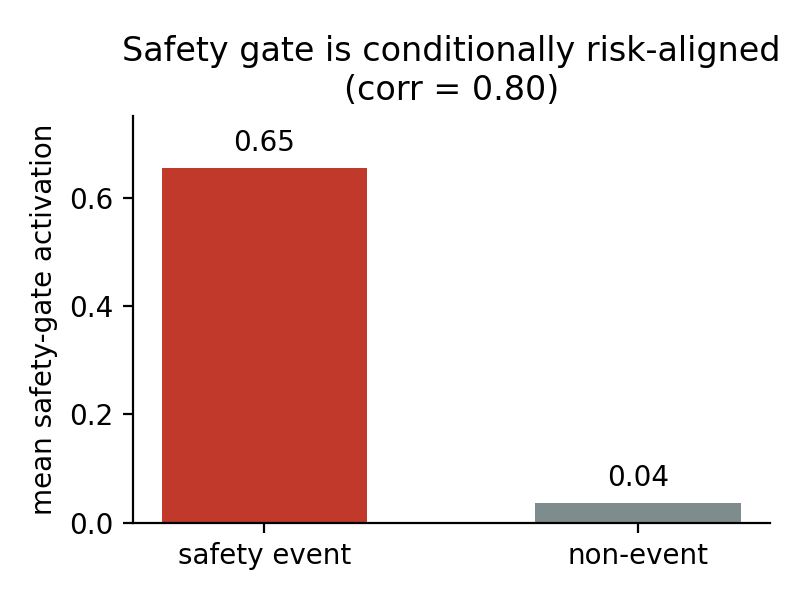
\includegraphics[width=0.46\linewidth]{figs/figA_safety_gate.png}
\caption{The safety gate activates on safety events (0.65) and stays quiet otherwise (0.04)---a
conditional, not constant, alignment (corr 0.80).}
\label{fig:gate}
\end{figure}

\textbf{The decisive variable is data, not architecture.} The same architecture yields correlation
$-0.03$ (\texttt{ce\_align\_all}) when the evaluated distribution lacks safety-positive samples, and
0.80 once safety-event collection and re-labeling are forced. H3 is \emph{unlocked by data
composition}; no architectural change is responsible. The transferable lesson: transparent routing
can be \emph{measured} and \emph{tied to real risk events}---but only if the data exposes those
events.

\textbf{Honesty.} The H3 evidence is primarily offline; baseline diversity is limited; a small
closed-loop check (seed 10) shows 0 collisions over short routes ($\sim$152\,m) but is not a driving
result. Part II is.

\section{Part II---Control Fails}
\textbf{From explanation to control.} We wrap the identical interpretable policy as a Bench2Drive-220
leaderboard agent and score it closed-loop. It scores \textbf{DS 0}: the router collapses
out-of-distribution to the legality expert (gate $\rightarrow [0,1,0,0]$), producing a constant brake.
Explanation quality does not transfer to control.

\textbf{A genuine recovery campaign.} We did not stop at the collapse. We ran, in order: (i)
teacher-data scale-up to \textbf{8{,}456 frames / 43 routes / 9 towns} (PDM-Lite~\cite{pdmlite}
teacher, failed-teacher runs excluded); (ii) loss balancing for mobility; (iii) a capacity increase
(wider router/expert MLPs); and (iv) a full \textbf{structural fork}---separating a mobility head from
a hazard-conditioned brake head, adding front-actor distance and closing speed to the input, and
retraining \textbf{from scratch} (no warm start) on the 8.4k data. Every candidate was judged
\emph{only} by closed-loop Driving Score.

\textbf{The seesaw.} No configuration reconciles safety and mobility. Table~\ref{tab:seesaw} traces
the tension on one representative route (24211): pushing the policy to move makes it collide; making
it safe makes it stop (Fig.~\ref{fig:seesaw}).

\begin{table}[ht]
\centering
\caption{Control: the safety/mobility seesaw at route 24211.}
\label{tab:seesaw}
\begin{tabular}{lrrr}
\toprule
Candidate & route \% & collisions & mean brake \\
\midrule
\texttt{scale\_b\_full}          & 3.08 & 0 & 0.586 \\
\texttt{scale\_b\_full\_go3}     & 100  & 3 & 0.022 \\
\texttt{scale\_b\_cap1\_balanced}& 4.59 & 0 & 0.205 \\
\texttt{struct\_sep\_fresh}      & 3.08 & 0 & 0.350 \\
\bottomrule
\end{tabular}
\end{table}

The structural fork---the strongest intervention---over-brakes on all three gate routes alike
(Table~\ref{tab:fork}): it reaches the goal of \emph{not colliding} only by \emph{not driving}.

\begin{table}[ht]
\centering
\caption{Structural fork (separated heads + hazard inputs + from-scratch): over-brake on all routes.}
\label{tab:fork}
\begin{tabular}{lrr}
\toprule
Route & route \% & collisions \\
\midrule
24211 & 3.08 & 0 \\
24240 & 4.05 & 0 \\
24330 & 4.05 & 0 \\
\bottomrule
\end{tabular}
\end{table}

\begin{figure}[ht]
\centering
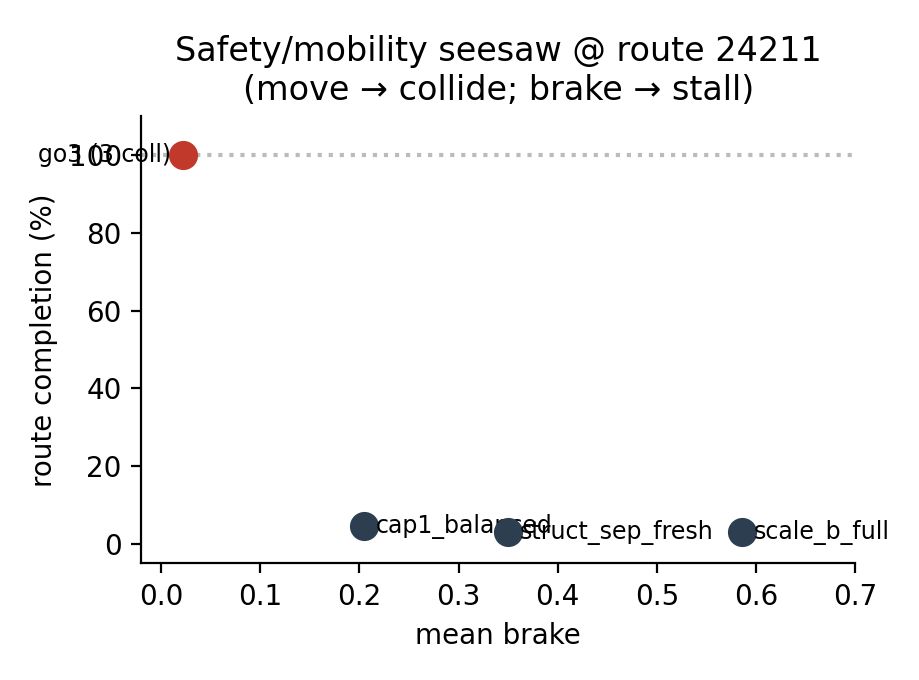
\includegraphics[width=0.52\linewidth]{figs/figB_seesaw.png}
\caption{Every candidate sits at an extreme of the brake axis: high brake $\Rightarrow$ stall
(route $\sim$3--5\%), low brake $\Rightarrow$ collisions. The middle (selective deceleration) is never
reached.}
\label{fig:seesaw}
\end{figure}

\textbf{Mechanism: fed but ignored.} The hazard evidence the brake head was supposed to use \emph{is
in the input}, yet the policy does not condition on it: within 10\,m of a front actor the mean
throttle is \textbf{0.93} and the mean brake \textbf{0.00}. The policy learns a \emph{global} brake
bias---turn it up and it over-brakes everywhere, turn it down and it collides---rather than a
\emph{conditional} response to the actual hazard. Two extremes are reachable; the middle is not.

\subsection{From escaping the over-brake to driving---and where it stops}
\textbf{Step 1: the over-brake was the learned brake.} We change the one thing that produced it: the
action head. The re-trained model (\emph{identical} data, router, experts, gate, and route inputs)
predicts steer and a forward command but \textbf{no brake}---the brake output is fixed to zero, so the
model cannot over-brake; braking is delegated to a standard safety shield. This alone is a controlled
change---only the action head's brake differs from the structural fork---and it lifts the three gate
routes from $\sim$3--4\% (Table~\ref{tab:fork}) to $\sim$46\% completion, collision-free on two of
three, with the agent never stalling.

\textbf{Step 2: a control stack drives---and generalizes to some unseen routes.} Pairing the learned
target speed with a classical longitudinal controller (a PID), the safety shield, and a small
anti-stall floor lets the policy actually drive. Of the five evaluation routes only 24211 appears in
the training data; the other four are \emph{unseen}. On an unseen route the policy drives cleanly end
to end (Table~\ref{tab:v2}): \textbf{route 24330 reaches 100\% completion with zero collisions and zero
lane departures}, and unseen 24240 reaches 53\% (there it is permanently blocked behind a scenario
obstacle that would require a lateral maneuver to pass).

\textbf{Step 3: but it does not generalize \emph{uniformly}.} Two other unseen routes reach only
18--25\% (Table~\ref{tab:v2}), with collisions and lane departures---and even the lone \emph{trained}
route, 24211, still collides at 88\%. So this is not a clean train/test overfitting gap (the cleanest
route is unseen; the trained route is not perfect) but a \emph{scenario-dependent} generalization gap:
the policy handles some unseen scenarios cleanly and mishandles specific hazards in others, as expected
for $\sim$8.5k frames over 43 routes with no on-policy data.

\begin{table}[ht]
\centering
\caption{X-MoD with the target-speed head + a classical control stack (PID, safety shield, anti-stall
floor). Cells are route completion \% (collision count). Of the five routes only 24211 is in training;
the other four are \emph{unseen}. The policy drives one unseen route cleanly (24330, 100\%/0, robust
across three traffic seeds) but mishandles specific hazards on others---a scenario-dependent gap, not a
clean train/test split (the trained route itself still collides).}
\label{tab:v2}
\begin{tabular}{lc|cccc}
\toprule
 & trained & \multicolumn{4}{c}{unseen} \\
 & 24211 & 24330 & 24240 & 24781 & 24841 \\
\midrule
completion \% (collisions) & 88 (1) & \textbf{100 (0)} & 53 (1) & 25 (1) & 18 (2) \\
\bottomrule
\end{tabular}
\end{table}

The honest reading is neither ``it drives'' nor ``it fails.'' With the control stack, the learned
target-speed policy drives an \emph{unseen} route cleanly to 100\%---a first for this model---yet
mishandles specific hazards on other unseen routes. The over-brake was the learned brake output; the
remaining wall is \emph{generalization to harder scenarios}, not the decomposition, and not a simple
train/test overfit (the cleanest route is unseen; the one trained route still collides). (Completion
comes from the policy \emph{plus} the standard control stack, not the policy alone; results are
single-checkpoint.)

\textbf{Robustness, and what does \emph{not} scale.} The 24330 result is not a lucky single run: it
holds at \textbf{100\% completion with zero collisions across three traffic-manager seeds}. The
per-route \emph{variation}, by contrast, tracks \emph{training composition} rather than eval noise.
Re-training on 11 of the 43 routes and re-evaluating the same unseen routes swings them widely (24330
$52\rightarrow100$, 24781 $81\rightarrow25$ as the training set grows $11\rightarrow43$), yet the
\emph{mean} unseen completion is essentially unchanged ($\approx$51\% at 11 routes vs.\ $\approx$49\% at
43). Quadrupling the training routes did not raise average generalization---it only redistributed which
unseen routes the brittle policy happens to transfer to. Nor does adding \emph{failure-correction} data
help: re-training with the available privileged-expert collision-source corrections (the kind of data
an on-policy DAgger loop would supply) \emph{lowers} held-out completion (mean $\approx$22\%
$\rightarrow$ $\approx$12\% with the failure states class-balanced, $\approx$8\% without) and degrades
steering, the safety-heavy failure states reintroducing the very over-caution we had removed. So the
residual is not a data-\emph{quantity} wall, and it is not closed by the failure-correction data at
hand; it is a composition/robustness problem that a small, single-camera policy does not absorb,
pointing to capacity and a \emph{carefully retained} on-policy loop rather than a quick data patch.

\section{Why: Readable Arbitration $\neq$ Drivable Arbitration}
\label{sec:why}
The arbitration signal that makes X-MoD \emph{explainable} (the gate) reads risk well, as Part I
shows. But reading risk is not the same as \emph{resolving} the safety$\leftrightarrow$mobility
conflict moment-to-moment, which is what control requires. The negative result localizes precisely
what is missing:
\begin{enumerate}[leftmargin=1.6em,itemsep=2pt]
  \item \textbf{A closed-loop learning loop.} Nothing updates the policy's priorities from the
  \emph{consequences} of its own closed-loop states; imitation on clean teacher data never sees the
  student's failure states (the classic compounding-error / distribution-shift wall).
  \item \textbf{Persistence / memory.} A conditional response to an unfolding hazard needs state that
  survives across timesteps; a single feed-forward pass does not carry it.
  \item \textbf{A monitor / ``pause.''} No layer watches the arbitration and \emph{interrupts} a bad
  trajectory; the gate explains but cannot veto.
\end{enumerate}
Crucially, a fourth factor turned out to be \textbf{dominant}: the action head's \textbf{brake output}.
The four candidates all emit a learned brake; zeroing it (Table~\ref{tab:v2}, with braking delegated to
a standard safety shield) removes the over-brake stall on the identical model and data. So the
over-brake seesaw was substantially an artifact of the learned brake output, \emph{not} of
interpretable decomposition. The three pieces above (loop, memory, monitor)---together with on-policy
data---are what the \emph{residual} failure now demands: with a control stack the policy drives some
\emph{unseen} routes cleanly (one to 100\%) but mishandles specific hazards on others, and that
scenario-dependent gap is exactly the distribution-shift the learning loop is meant to close. They are
no longer needed to explain the over-brake corner, which the brake output alone accounts for.

\section{Limitations and Non-claims}
\textbf{Claimed:} (i) under \emph{direct pedal regression}, an interpretable Mixture-of-Drives exhibits
a reproducible over-brake/collision seesaw that survives data scale, loss balancing, width, and
structural separation; (ii) removing the model's learned brake output (an action head with no brake)
and pairing the learned target speed with a classical control stack (PID, safety shield, anti-stall
floor)---changing neither the decomposition nor the data---lets the policy \emph{complete} an
\emph{unseen} route (24330: 100\%, zero collisions, \emph{across three traffic seeds}; only 24211 of
the five eval routes is in training).
\textbf{Not claimed:} that this model \emph{drives} Bench2Drive in general---it does \emph{not}
generalize uniformly: other unseen routes reach only 18--25\% with collisions (and the lone trained
route still collides at 88\%), a scenario-dependent generalization gap rather than a clean train/test
overfit; nor that the decomposition itself \emph{helps} driving; nor that the gap is closed by
\emph{quantity}---a scaling probe ($11\rightarrow43$ training routes) left mean unseen completion
unchanged ($\approx$51\%~$\rightarrow$~$\approx$49\%). The Part~I explanation result is primarily
offline; runtime inputs are non-privileged; \textbf{completion comes from the learned policy
\emph{plus} a standard control stack} (PID + safety/anti-stall shields), not the policy alone; results
are single-checkpoint (the 24330 milestone is three-seed).

\section{Future Work---Toward Drivable Arbitration}
The results set a sharp coordinate. The over-brake corner is solved by removing the learned brake, and
the policy already drives an \emph{unseen} route cleanly to 100\%. The residual wall is
\textbf{scenario-dependent generalization}: other unseen routes reach only 18--25\%, the signature of
pure imitation on $\sim$8.5k frames over 43 routes. Closing it is the harder road---on-policy data
(DAgger over the policy's own closed-loop states), more teacher data, and a lateral re-parametrization
(waypoints + a classical lateral controller) for the steering errors that dominate the failing routes. The longer
arc---a closed-loop learning loop, persistence, and a monitoring ``pause''---is precisely what turns a
trustworthy arbitration \emph{signal} into a \emph{generalizing} controller. The claims of \emph{this}
paper remain restricted to the measured results above.

\section{Conclusion}
``Readable'' and ``drivable'' are not the same property---and for this interpretable policy, the gap
between them was mostly its \emph{learned brake output}, not the decomposition. Remove that brake and
add a classical control stack, and the transparent arbitrator that explains risk faithfully
(correlation 0.80) actually \emph{drives}: it completes an \emph{unseen} route at 100\% with zero
collisions. But it does not generalize uniformly---other unseen routes reach only 18--25\%, and even
the one trained route still collides. The honest verdict is neither ``it fails'' nor ``it drives'' but
a located one: the decomposition was never the blocker; the over-brake was the learned brake, and what
now stands between this policy and Bench2Drive is \emph{generalization to harder scenarios}.

\bibliographystyle{plain}
\bibliography{references}

\end{document}
